% !TEX program = xelatex
% !TeX encoding = utf8
% !TeX spellcheck = pl-PL

%%%%%%%%%%%%%%%%%%%%%%%%%%%%%%%%%%%%%%%%%%%%%%%%%%%%%%%%%%%%%%%%%%%%%%%%%%%
% Wybierz rodzaj pracy dyplomowej oraz wydział
% Pick thesis type and faculty
%%%%%%%%%%%%%%%%%%%%%%%%%%%%%%%%%%%%%%%%%%%%%%%%%%%%%%%%%%%%%%%%%%%%%%%%%%%
\documentclass[thesis=inz,faculty=ee]{EE-dyplom} 
\usepackage{mwe}
\usepackage{graphicx}
\usepackage{float}
\usepackage{caption}


% thesis=[inz|mgr|bsc|msc]
%  * inz - praca inżynierska
%  * mgr - praca magisterska
%  * bsc - bachelor thesis
%  * msc - master thesis

% Skróty nazw wydziałów zgodne z domenami internetowymi
% Abbreviations of Faculties according to Internet subdomains
% faculty=[
%	arch,
%	gik,
%	ee,
%	wip
%	]

%%%%%%%%%%%%%%%%%%%%%%%%%%%%%%%%%%%%%%%%%%%%%%%%%%%%%%%%%%%%%%%%%%%%%%%%%%%
% Konfiguracja - do personalizacji
% Configuration - to be personalized
%%%%%%%%%%%%%%%%%%%%%%%%%%%%%%%%%%%%%%%%%%%%%%%%%%%%%%%%%%%%%%%%%%%%%%%%%%%
\instytut{}
\kierunek{Informatyka Stosowana}
\specjalnosc{Inżynieria Oprogramowania}
\title{Oprogramowanie wykrywające ataki typu ransomware na podstawie analizy statystyk generowanych przez system plików}
\engtitle{Software to detect ransomware attacks based on analysis of statistics generated by the file system}
\album{311351}
\author{Maciej Michalski}
\promotor{dr inż. Radosław Roszczyk}
\date{2023}
\longdate{2023-XX-XX}

%\grantlicense{TRUE} % [TRUE|FALSE]

%%%%%%%%%%%%%%%%%%%%%%%%%%%%%%%%%%%%%%%%%%%%%%%%%%%%%%%%%%%%%%%%%%%%%%%%%%%
% Streszczenie pracy i abstract.
% In case of thesis in English swap the order - English version goes first.
%%%%%%%%%%%%%%%%%%%%%%%%%%%%%%%%%%%%%%%%%%%%%%%%%%%%%%%%%%%%%%%%%%%%%%%%%%%
\streszczeniepracy{
Tutaj znajdować się będzie streszczenie
\lipsum[1-4]
} % koniec streszczenia

\slowakluczowe{ransomware, administracja, cyberbezpieczeństwo}

\thesisabstract{
Here will be an abstract of the paper
\lipsum[1-4]
} % end of abstract

\thesiskeywords{ransomware, administration, cybersecurity}

%%%%%%%%%%%%%%%%%%%%%%%%%%%%%%%%%%%%%%%%%%%%%%%%%%%%%%%%%%%%%%%%%%%%%%%%%%%
% Tu zaczyna się dokument
% Here is the beginning of the document
%%%%%%%%%%%%%%%%%%%%%%%%%%%%%%%%%%%%%%%%%%%%%%%%%%%%%%%%%%%%%%%%%%%%%%%%%%%
\begin{document}
    % Strony nagłówkowe
    % Headers
    \frontpages

    % Właściwa treść jest w pliku tekst/main.tex
    % Real contents is in tekst/main.tex
    % Rozdziały zaczynają się od "chapter"
\chapter{Wprowadzenie}
% Praca podzielona na mniejsze pliki włączane za pomocą input
% Zajrzyj do pliku tekst/wstep.tex
Głównym celem każdej aplikacji cyfrowej, systemu informatycznego czy innego rodzaju usług dostępnych przez sieć jest przetwarzanie informacji cyfrowej. Dzięki dygitalizacji usług oraz utworzeniu kompletnie nowych jej rodzajów zależnych od technologii cyfrowych ludzkość generuje masywne ilości danych każdego dnia. Jednym~z~najpopularniejszych środków komunikacji, zwłaszcza dla biznesu, jest poczta elektroniczna. Grupa \textbf{Radicati Inc.} spekuluje, że do końca 2023 liczba wysłanych listów elektronicznych powinna przekroczyć 347 miliardów \cite{radicati2019}.
\textbf{Domo, Inc}, które jest jednym~z~wielu dostawców usług chmurowych,~w~swoim raporcie zatytułowanym 
\foreignquote{english}{Data Never Sleeps 10.0} donosi o tym, że wielkość danych, które zostaną utworzone czy skopiowane może wejść~w~okolicę 181 zettabajtów\footnote{Zetta bajt (skrót \textbf{ZB})~w~systemie SI to tryliard $10^{21}$ bajtów~i~$2^{70}$, czyli $1024^{7}$ bajtów.} wielkości do roku 2025 \cite{domo10}. Znakomita część tych danych musi być przechowywana na stałe, gdyż wymaga tego poprawne działanie systemu lub może wynikać~z~nakazów prawnych.~Z~tych powodów jednym~z~priorytetów przy administracji systemu jest zabezpieczenie przed utratą danych przez instytucje~i~działalności gospodarcze.
Do powodów utraty danych mogą należeć:
\begin{itemize}
    \item awaria nośników~i~innych elementów,
    \item niespodziewane braki~w~dostawach prądu,
    \item błąd ludzki,
    \item wirusy komputerowe.
\end{itemize}

%%%%%%%%%%%%%%%%%%%%%%%%%%%%%%%%%%%%%%%%%%%%%%%%
\section{Cel pracy}
Celem tej pracy było odnalezienie sposobu na zniwelowanie strat danych~w~wyniku ataku wirusa typu ransomware możliwego do wykorzystania przez administratorów~w~warunkach rzeczywistego ataku. Zaproponowanym przeze mnie rozwiązaniem jest \foreignquote{english}{proof of concept} w postaci oprogramowania analizującego działania na plikach dla systemów operacyjnych~z~rodziny Linux.
%Celem tej pracy było utworzenie oprogramowania, które zajmuje się niwelowaniem ryzyka utraty danych~z~powodu ataku wirusa komputerowego typu ransomware na systemach~z~rodziny Linux oraz przetestowanie jego działania~w~trakcie rzeczywistego ataku.
 Program korzysta~z~informacji o stanie systemu plików~i~na bieżąco analizuje wykonywane na nim operacje. Statystyki~z~obserwowanego obszaru zawierają~w~sobie m.in. ilości operacji, ścieżkę do użytej komendy, nazwę użytkownika, który dokonuje operacji etc. Dzięki temu administrator może nie tylko dowiedzieć się o potencjalnym zagrożeniu ataku ransomware, ale też obserwować dowolny, podejrzany ruch na systemie plików. Następnie dokonywana jest analiza zawartości plików~i~generowany jest raport o zakresie ryzyka.
Docelową grupą użytkowników są administratorzy,~a~więc główne założenia, jakie postawiłem sobie~w~trakcie tworzenia rozwiązania, miały na celu wytworzenie oprogramowania łatwego dla nich~w~obsłudze. Tymi założeniami są:
\begin{itemize}
    \item łatwa instalacja, która nie wymaga aktualizacji sterowników sprzętowych,
    \item wsparcie dla najpopularniejszych dystrybucji serwerowych\footnote{W3 Techs utrzymuje raport o sieciowych serwerach Linuksowych. Jest on codziennie aktualizowany~i~można go odnaleźć pod adresem: \url{https://w3techs.com/technologies/details/os-linux}},
    \item minimalne zużycie zasobów,
    \item integracja~z~bieżącymi popularnymi rozwiązaniami~w~administracji systemów.
\end{itemize}

%%%%%%%%%%%%%%%%%%%%%%%%%%%%%%%%%%%%%%%%%%%%%%%%
\section{Opis problemu~i~znaczenie zagrożeń typu ransomware}
 Od 2017 roku obserwuje się trend wzrostowy ataków ransomware\cite{petrosyan_worldwide_nodate}, a~w~ciągu pierwszej połowy 2022 roku, dokonano 236,7 miliona ataków na całym świecie 
 \cite{petrosyan_number_nodate}. Wg. raportu Verizona \footnote{Raport jest odpłatnie dostępny pod linkiem: \url{https://www.verizon.com/business/resources/reports/dbir/2021/results-and-analysis}} ataki ransomware stanowią 10\% wszystkich naruszeń danych~w~2021. Wedle zebranych statystyk wykrycie ich zajęło~w~aż 49 dni dłużej niż średni czas wykrycia wszystkich naruszeń~z~tego samego roku. Raport wyjaśnia też, że zagrożona nie jest wyłącznie branża IT, ale też inne sektory,~w~szczególności sektor ochrony zdrowia.
\begin{figure}[H]
     \centering
     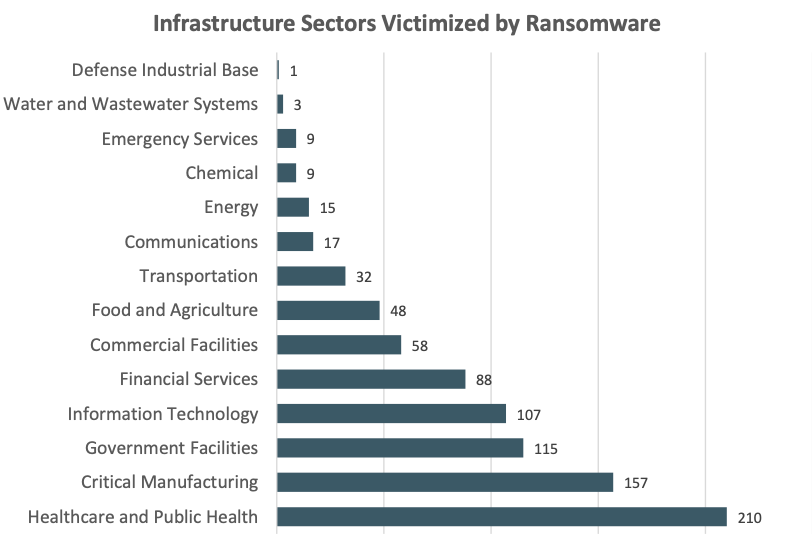
\includegraphics[width=0.78\linewidth]{rysunki/attacks_on_sectors.png}
     \caption{Sektory infrastruktury krytycznej, do których odnosiły się skargi IC3\protect\footnotemark.}
     \label{fig:enter-label}
 \end{figure}
\footnotetext{\emph{FBI 2022 Internet Crime Report}, s. 14}

 Raport IC3~z~roku 2022 donosi o 870 zarejestrowanych skargach dotyczących ataków, których celem były organizacje infrastruktury krytycznej. Pośród 16 sektorów, 14~z~nich padło ofiarą próby ataku.
  \begin{figure}[H]
     \centering
     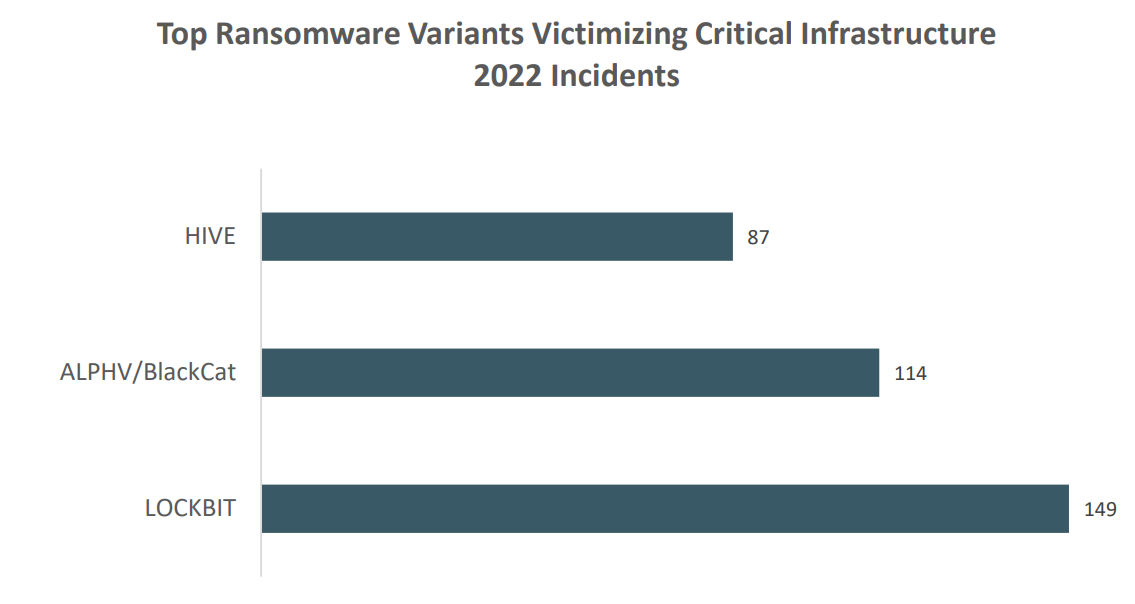
\includegraphics[width=0.75\linewidth]{rysunki/topransomwares2022.png}
     \caption{Najpopularniejsze warianty wirusów ransomware, zarejestrowane~w~trakcie incydentów mających na celu atak infrastruktury krytycznej. Należy zauważyć, że wirus \foreignquote{english}{LockBit} sprawiał najwięcej problemów. Jego wersja na system Linux nosi nazwę \foreignquote{english}{LockBit Linux-ESXi Locker }\protect\footnotemark.}
     \label{fig:enter-label}
 \end{figure}
 \footnotetext{\emph{FBI 2022 Internet Crime Report}, s. 15}

 Raport grupy \foreignquote{english}{Herjavec} donosi, że aż 70\% organizacji medycznych borykało się~z~poważnymi komplikacjami przez ataki ransomware \cite{health}.
~W~2022 roku 1 na 42 instytucje ochrony zdrowia były ofiarami tychże ataków, 74\%~z~nich to szpitale 
 \cite{etal_check_2022}.
 \begin{figure}[H]
    \centering
    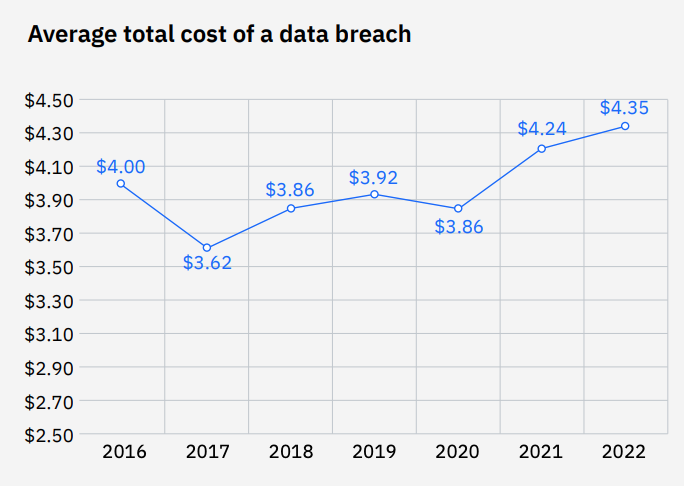
\includegraphics[width=0.7\linewidth]{rysunki/costOfDataBreach.png}
    \caption{Średni koszt naruszenia danych 2016-2022\protect\footnotemark.}
    \label{fig:enter-label}
\end{figure}
\footnotetext{\emph{Cost of~a~Data Breach
Report 2022}, figure 1, s. 9.}

~Z~danych zebranych~z~ostatnich 5 lat jednoznacznie wynika, że nieumiejętne przeciwdziałanie może zaszkodzić nie tylko finansom zaatakowanej działalności lub osoby indywidualnej, ale również stwarza zagrożenie dla zdrowia~i~życia.
 Dodatkowo, mając na uwadze średni koszt naruszenia danych~w~2023, którego globalna średnia wynosi 4,45 milionów USD \cite{petrosyan_global_cost},
 coraz więcej administratorów jest zmuszonych dywersyfikować sposoby zabezpieczania systemów. 
 \begin{figure}[H]
     \centering
     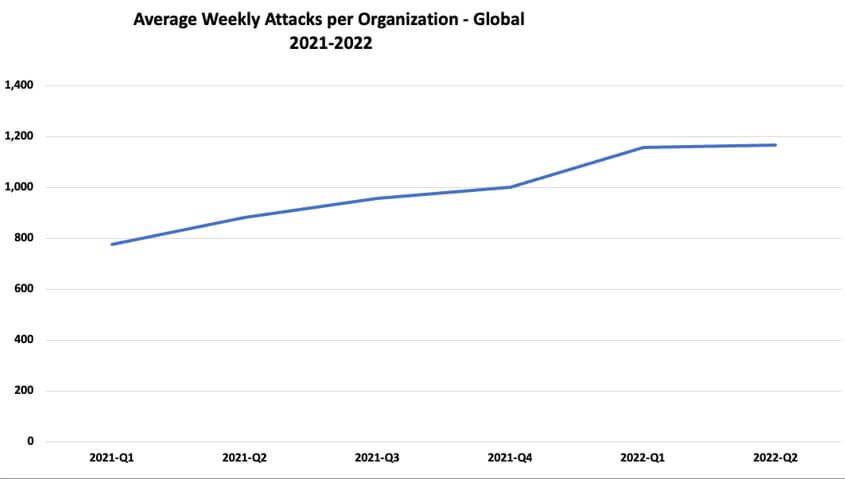
\includegraphics[width=0.75\linewidth]{rysunki/Global-Quarterly-attacks-from-Q1-2021- Q2-2022.png}
     \caption{Globalnie zgłoszone incydenty ataków ransomware per kwartał~w~roku 2022 zarejestrowanych przez Check Point Research. Organizacja spekuluje, że wzrost ataków mógł być spowodowany lukami bezpieczeństwa \foreignquote{english}{log4j} oraz cyberataków związanych~z~wojną~w~Ukrainie\protect\footnotemark.}
     \label{fig:enter-label}
 \end{figure}
\footnotetext{\emph{Check Point Research: Weekly Cyber Attacks increased by 32\% Year-Over-Year; 1 out of 40 organizations impacted by Ransomware}, figure 1.}

 Na rynku istnieje wiele popularnych rozwiązań działających prewencyjnie m.in.~w~tym rozbudowane aplikacje służące do tworzenia~i~przywracania kopii zapasowych. Należy jednak wziąć pod uwagę, że przywracanie danych nie jest prostym procesem.~W~zależności od rodzaju użytego nośnika przywracanie może doprowadzić nawet do przypadkowej utraty danych przy zniszczeniu nośnika danych~w~przypadku taśm. Jest to także proces powolny, co~w~efekcie może spowodować poniesienie większych kosztów niż wartość okupu.
 \newline
 Rozwiązaniem, które wydaje się być aktualnie najlepszym, jest możliwie jak najwcześniejsze wykrycie potencjalnego źródła ataku.~W~przypadku, gdy te czynności zawiodą, jedyną możliwością na zmniejszenie strat jest minimalizacja skutków ataku na bieżąco. Aby tego dokonać, konieczne jest wczesne wykrycie ataku.
 
\begin{figure}[H]
\centering
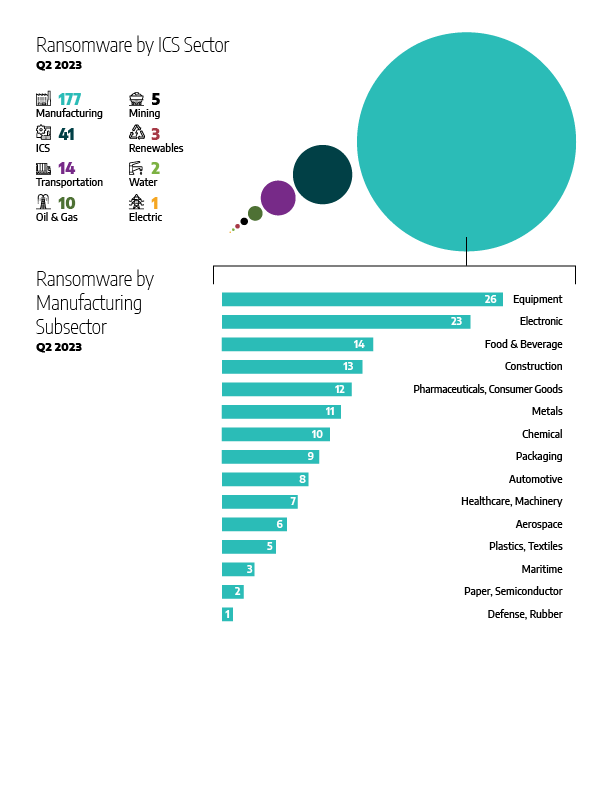
\includegraphics[width=0.6\linewidth]{rysunki/attackbysector.png}
\caption{Incydenty ransomware per sektor gospodarki\protect\footnotemark. }
\label{fig:enter-label}
\end{figure}
\footnotetext{\emph{Dragos Industrial Ransomware Attack Analysis: Q2 2023}, figure 2.}


%%%%%%%%%%%%%%%%%%%%%%%%%%%%%%%%%%%%%%%%%%%%%%%%
\section{Krótka charakterystyka ataków ransomware}
Ransomware można zdefiniować jako oprogramowanie, które blokuje atakowanemu dostęp do danych, do momentu zapłacenia okupu \cite{ransomware_us}. Prostsze ataki mogą sprowadzać się do blokady systemu bez uszkadzania plików, jednak większym zagrożeniem są tzw. \foreignquote{english}{cryptovirological attacks} \cite{502676}, czyli ataki wykorzystujące szyfrowanie danych jako formę blokady danych. Atakowany, jeśli nie posiada kopii zaszyfrowanych danych, musiałby odnaleźć klucz, którego użyto~w~szyfrowaniu. Nawet jeśli atakowany wie jakiego algorytmu użyto~w~ataku, to odnalezienie klucza jest problemem trudnym, zwłaszcza dla nowoczesnych algorytmów szyfrowania. Przykładowo, algorytm \foreignquote{english}{AES}~w~zależności od klucza występuje~w~wariantach 128,192 oraz 256-bitowych, co daje między $2^{128}$~a~$2^{256}$ możliwych wartości do sprawdzenia atakiem siłowym. 
\newline
Przy wyłudzaniu okupu, atakujący stosują również techniki zastraszenia. Przykładowo wirus \foreignquote{english}{WannaCry}, którego duża fala ataków miała miejsce~w~2017 roku \cite{czarnecki_oto_2017}, informował, że początkowy okup 300\$ per maszyna wzrośnie dwukrotnie po 3 dobach zwłoki. Po upływie tygodnia odzyskanie danych miałoby stać się niemożliwe. Atakujący wymagają, aby okup został spłacony~w~sposób trudny do wyśledzenia przez organy ścigania m.in. za pomocą kryptowalut.
\begin{figure}[H]
    \centering
    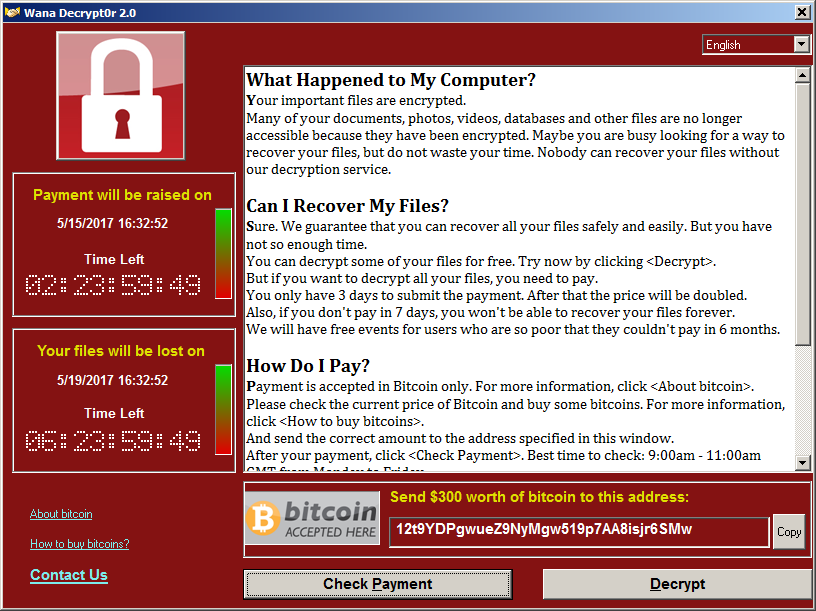
\includegraphics[width=0.8\linewidth]{rysunki/wannacry.png}
    \caption{Ekran wyświetlający się po zainfekowaniu komputera przez WannaCry. Atakujący wymaga od ofiary zapłaty Bitcoinem\protect\footnotemark.}
    \label{fig:enter-label}
\end{figure}
\footnotetext{\url{https://www.galsys.co.uk/news/wp-content/uploads/WannaCry-Pop-Up.jpg}}

Ataki ransomware, mogą także założyć blokadę powłoki systemowej lub nawet dokonać modyfikacji partycji rozruchu jak~w~przypadku wirusa RedBoot \cite{redboot}.

\begin{figure}[H]
    \centering
    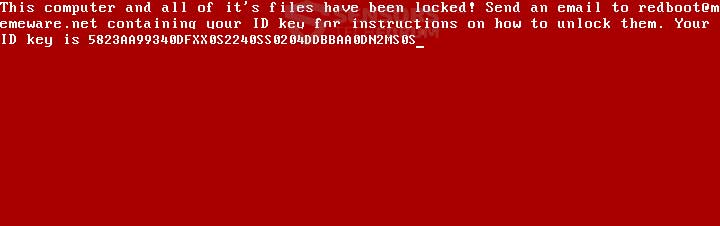
\includegraphics[width=0.95\linewidth]{rysunki/redboot.png}
    \caption{Ekran rozruchu przy infekcji wirusem RedBoot\protect\footnotemark.}
    \label{fig:enter-label}
\end{figure}
\footnotetext{\url{https://www.bleepstatic.com/images/news/ransomware/r/redboot/header.png}}

Konceptualnie \foreignquote{english}{cryptovirological attack} został przedstawiony~w~1996 roku na konferencji IEEE Security \& Privacy~\cite{yung}. Opisuje się go jako protokół pomiędzy atakowanym,~a~atakującym:

\begin{figure}[H]
    \centering
    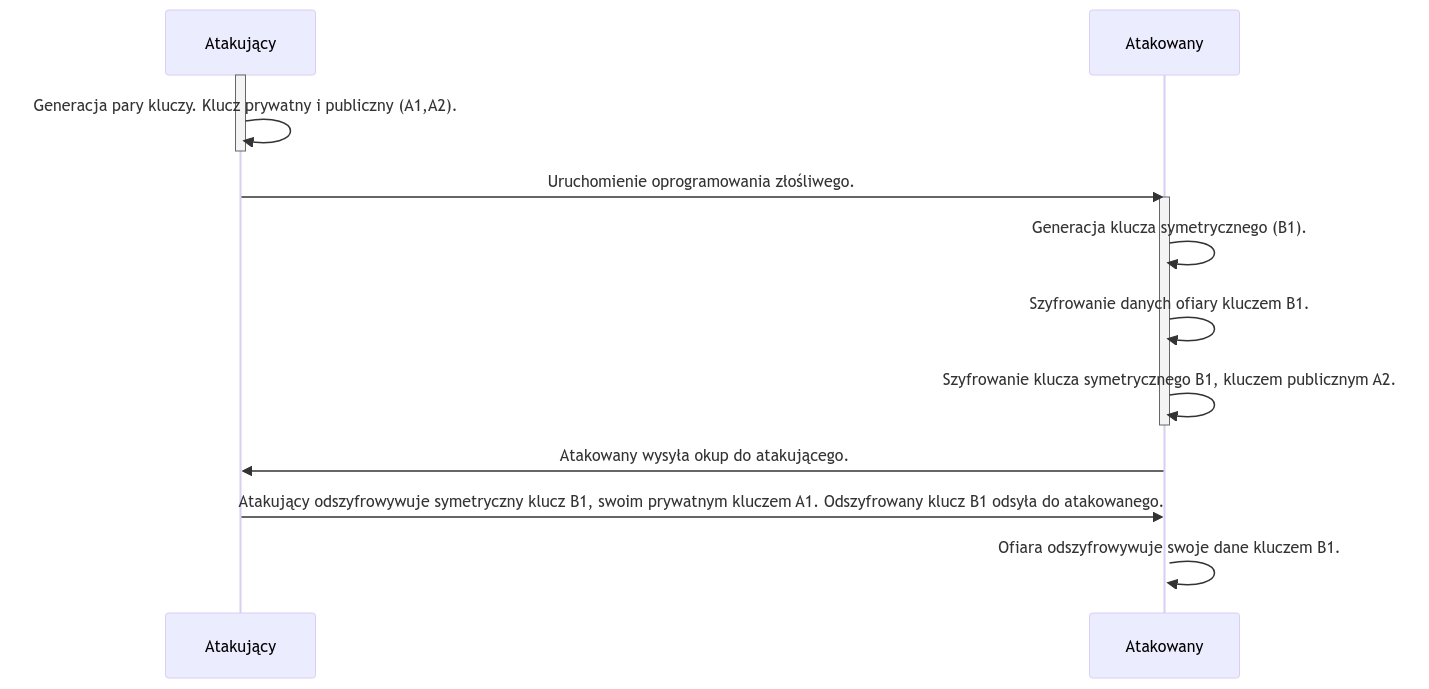
\includegraphics[width=1\linewidth]{rysunki/sequenceRansomware.png}
    \caption{Diagram sekwencji ataku ransomware.}
    \label{fig:enter-label}
\end{figure}
Generowany klucz symetryczny ma charakter losowy~i~nie pomoże~w~odszyfrowaniu danych innej ofiary. Klucz prywatny jest przechowywany wyłącznie przez atakującego. Jedyny kontakt, jaki musi być wykonany bezpośrednio przez atakującego, następuje~w~momencie kiedy zaszyfrowany klucz symetryczny jest wysyłany do atakującego,~a~następnie klucz odszyfrowany do atakowanego.
\newline
Typowymi sposobami propagacji ransomware są:
\begin{itemize}
    \item podszywanie się pod znane aplikacje czy strony internetowe,
    \item skuszenie ofiary do otworzenia niezaufanego załącznika listu elektronicznego,
    \item luki bezpieczeństwa sieci.
\end{itemize}

%%%%%%%%%%%%%%%%%%%%%%%%%%%%%%%%%%%%%%%%%%%%%%%%

% Można też wszystko pisać w jednym pliku ale będzie on duży
\chapter{Przegląd literatury}
% fragment nieużywany albo jeszcze niedodany można zakomentować
W artykule opublikowanym przez firmę Microsoft\footnote{Artykuł jest dostępny pod adresem: \url{https://www.microsoft.com/pl-pl/security/business/security-101/what-is-cybersecurity}} o tytule \enquote{Co to jest cyberbezpieczeństwo ?}, trzy z sześciu wymienionych typów zagrożenia to: 
\begin{itemize}
    \item oprogramowanie wymuszające okup,
    \item inżynieria społeczna,
    \item wyłudzanie informacji.
\end{itemize}
Atak ransomware zawiera w sobie każde z tych zagrożeń.
Oprogramowanie złośliwe wymaga od ofiary zaufania, że to co uruchamia jest nieszkodliwe. Typowo propagacja takiego malware ma miejsce poprzez tzw. 
\foreignquote{english}{phishing} czyli podszywanie się atakującego za zaufany serwis lub instytucję z którymi ofiara mogła wejść w interakcję w przeszłości. 
Aby zrozumieć zakres tych technik oraz możliwe wektory ataku, należy prześledzić ich historię.
%%%%%%%%%%%%%%%%%%%%%%%%%%%%%%%%%%%%%%%%%%%%%%%%
\section{Historia i ewolucja ataków typu ransomware}
\label{sec:his}
\subsection{Wczesna historia}
Mimo stopniowego nasilania się ataków ransomware w przeciągu ostatnich 7 lat sama idea utrudnienia
dostępu do plików pod groźbą okupu jest znana od dosyć dawna. Już w drugiej połowie lat 80-tych, w~USA,
cyberprzestępcy w zamian za odzyskanie dostępu do danych wyłudzali okup, który następnie był wysyłany drogą pocztową. Jednym z pierwszych udokumentowanych ataków wirusem ransomware był DOSowy \foreignquote{english}{AIDS trojan}~\cite{virus_1990} z 1989 roku. Autor programu — Joseph Popp — przekazywał dyskietki drogą pocztową do wybranej grupy ofiar pod przykrywką załącznika do ulotki informacyjnej na temat wirusa AIDS. Program modyfikował plik \texttt{AUTOEXEC.BAT}, z którego korzystał w celu zliczenia ilości uruchomień komputera. W momencie przekroczenia liczby 90 uruchomień szyfrował nazwy wszystkich plików na dysku \texttt{C:\/}, tym samym uniemożliwiając korzystanie z systemu.

\begin{figure}[H]
    \centering
    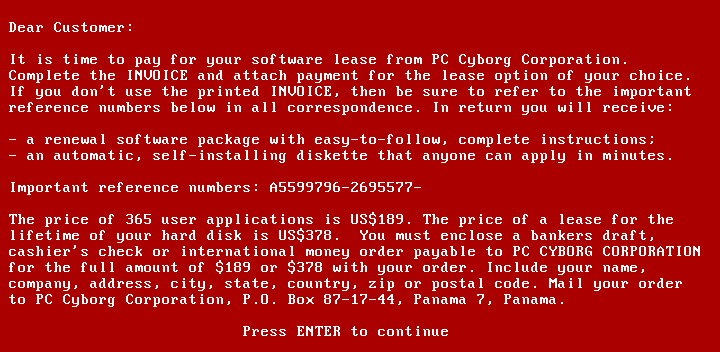
\includegraphics[width=0.6\linewidth]{rysunki/aids-trojan.png}
    \caption{Wiadomość ukazująca się po aktywacji wirusa \foreignquote{english}{AIDS trojan}\protect\footnotemark}
    \label{fig:enter-label}
\end{figure}
\footnotetext{\url{https://sophosnews.files.wordpress.com/2012/09/aids-info-demand-500.png}}

Atakujący podszywał się pod fikcyjną korporację \foreignquote{english}{PC Cyborg Corporation}, na której adres w~Panamie miał być wysyłany okup. Paczka razem z dyskietką posiadała również ulotkę z krótkim wprowadzeniem, instrukcją obsługi, a także licencją co było w tamtym czasie powszechną~i~budzącą zaufanie praktyką. 
Program nie szyfrował treści samych plików, jedynie ich nazwy. Klucz szyfrowania był kluczem symetrycznym, co sprawiało, że złamanie go mogło pomóc odblokować system, każdej ofierze borykającej się z tą samą wersją wirusa. Eliminacja tej wady była inspiracją dla pracy \foreignquote{english}{Cryptovirology: Extortion-Based Security Threats and Countermeasures}, w której przedstawiono pojęcie \foreignquote{english}{cryptovirological attack}~\cite{yung}.
\newline
Po roku 1996, w erze upowszechnienia się internetu, pojawiły się sporadyczne ataki ransomware na niewielką skalę, tym razem ulepszone o szyfrowanie hybrydowe. W latach dwutysięcznych pojawił się trudny do wykrycia \foreignquote{english}{PGPCoder}~\cite{tromer_cryptanalysis_nodate} używający 660-bitowego klucza RSA. Innym ransomware występującym w tamtym czasie był \foreignquote{english}{Archievus} ~\cite{arhiveus}, również używający klucza RSA, w wersji 1024-bitowej, którego tragiczną wadą było używanie tego samego klucza do szyfrowania każdego pliku na każdej zainfekowanej maszynie. Ataki te, aby zainfekować ofiarę, wykorzystywały phishing i~podszywały się pod zaufane strony internetowe. 
%%%%%%%%%%%%%%%%%%%%%%%%%%%%%%%%%%%%%%%%%%%%%%%%
\subsection{Historia współczesna}
Mimo historii sięgającej jeszcze lat 80 - tych, ataki ransomware nie były szczególnie powszechne w latach dwutysięcznych. Status quo został zachwiany po upowszechnieniu się kryptowalut, umożliwiających poufną~i~trudną do wyśledzenia wymianę środków między ofiarą a atakującym. Jednak uzyskanie pieniędzy od ofiar niezaznajomionych z kryptowalutami nie było proste, dopiero kantory kryptowalut dały cyberprzestępcom możliwość prostego~i~poufnego wyłudzenia środków. Pierwsza dekada XXI w. była dla cyberprzestępców czasem udoskonalania \foreignquote{english}{scareware}, czyli oprogramowania mającego wystraszyć ofiarę na tyle, żeby zapłaciła za odzyskanie dostępu do stacji, bez wyrządzania szczególnej szkody na danych. 
\newline
W 2013 roku w annały historii internetu wszedł Windowsowy wirus \foreignquote{english}{CryptoLocker}. Wykorzystywał on do szyfrowania 2048-bitową parę kluczy RSA, generowaną na osobnym serwerze, a następnie dostarczał klucz publiczny na stację ofiary w celu szyfrowania jej plików~\cite{cryptolockerfaq}. Tym samym ofiara nie miała innej możliwości odzyskania plików niż zapłacić okup wynoszący 300 USD. Wirus dostarczany był jako załącznik w liście elektronicznym oraz przez owiany złą sławą \foreignquote{english}{Gameover ZeuS botnet}~\cite{zeusbot}. Załącznik posiadał w sobie plik \texttt{.zip}, który z kolei zawierał w sobie plik \texttt{.exe}, z ikonką charakterystyczną dla pliku pdf. Atakujący wykorzystywał domyślne zachowanie Windowsa polegające na ukrywaniu rozszerzenia pliku. Następnie wirus podejmował następujące kroki:
\begin{enumerate}
    \item rozpakowywał swoje pliki w ścieżce profilu użytkownika,
    \item dodawał nową pozycję do windowsowego rejestru, który uruchamiał wirus wraz z rozruchem systemu,
    \item pobierał klucz publiczny z jednego z serwerów,
    \item wirus inicjował szyfrowanie plików na zamontowanych dyskach, w tym na dyskach sieciowych,
    \item wyświetla ekran informujący o zdarzeniu~i~możliwości opłacenia okupu w BTC do 100 godzin od zaszyfrowania.
\end{enumerate}
Po opłaceniu okupu ofiara miała możliwość pobrania programu dekodującego z załadowanym, odpowiednim kluczem prywatnym. Wirus szyfrował jedynie pliki z odpowiednimi rozszerzeniami m.in. pliki AutoCAD czy dokumenty MS Office.
\begin{figure}[H]
    \centering
    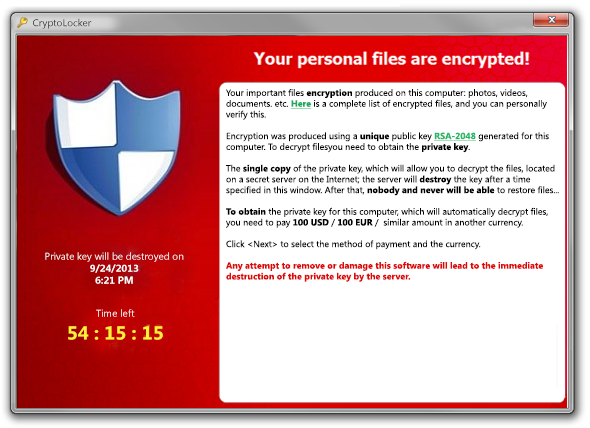
\includegraphics[width=0.75\linewidth]{rysunki/cryptolocker.png}
    \caption{Ekran wyświetlający się po zainfekowaniu komputera przez CryptoLocker\protect\footnotemark.}
    \label{fig:enter-label}
\end{figure}
\footnotetext{\url{https://grzegorzkowalik.com/wp-content/uploads/2015/05/cryptolocker.png}}
Zagrożenie tym wirusem zostało zneutralizowane w wyniku zainicjowanej przez departament sprawiedliwości USA, operacji \foreignquote{english}{Tovar}~\cite{tovar} w wyniku której udało się uzyskać dostęp do bazy danych zawierającej prywatne klucze RSA na podstawie których możliwe było odzyskanie plików.
\newline
\foreignquote{english}{CryptoLocker} był swego rodzaju kamieniem milowym w rozwoju cyberprzestępczości. Złożona natura procederu stała się normą dla ataków ransomware a wraz z coraz większą popularnością kryptowalut~i~usprawnionymi algorytmami szyfrowania asymetrycznego, ilość ataków oraz generowane przez nie straty stabilnie wzrastają aż do dnia dzisiejszego.
\newline
Aktualnie cyberprzestępcy zmienili styl ataku ze skupiającego się na infekcji jak największej ilości stacji, na tzw. \foreignquote{english}{big game hunting} (BGH)\footnote{Dokładniejszą definicję z przykładami można znaleźć pod adresem:\newline \url{https://www.malwarebytes.com/blog/news/2023/07/ransomware-making-big-money-through-big-game-hunting}}.  w dużej mierze polega na koordynacji inżynierii społecznej~i~zaprojektowania oprogramowania ransomware w sposób, który będzie najbardziej szkodliwy dla dużych organizacji. Obierana jest mniejsza ilość celów na rzecz wyższej kwoty okupu. Raport \foreignquote{english}{CrowdStrike Services} z 2023 roku donosi, że jedną najszerzej stosowanych taktyk BGH jest połączenie ransomware z groźbą upublicznienia skradzionych danych. Typowo dane zostają upubublicznione gdy minie termin zapłaty okupu. Naruszenie danych jest rozłożone w czasie~i~wykorzystuje narzędzia już dostępne na atakowanym środowisku. Dzięki temu ataki są cięższe do wykrycia\footnote{Technika ta nosi nazwę \foreignquote{english}{Living off the land}}.
Techniki zastraszenia zostały także dopracowane, aby wywołać możliwie na największą presję na ofiarach. W przypadku \foreignquote{english}{REvil} kradzione dane bywały etapowo upubliczniane, aby zmusić ofiarę do szybszego działania ~\cite{hern_ransomware_2021}.\newline
Z powodu dużej opłacalności takich ataków utworzony został model \foreignquote{english}{ransomware as a service} (RaaS), w którym klienci płacą za dokonanie ataku ransomware programem utworzonym przez inne grupy hakerskie\footnote{Wykorzystywane jest oprogramowanie utworzone przez inne osoby, podobnie jak w modelu Software as a Service.}. 
\newline
Jednym z nich jest wcześniej wymieniony \foreignquote{english}{REvil} używany przez grupę \foreignquote{english}{PINCHY SPIDER}, którego cechą rozpoznawczą jest postowanie skradzionych danych na blogu \foreignquote{english}{Happy Blog}~\cite{hern_ransomware_2021}. W 2021 roku użyto go na wysoką skalę~\cite{mcmillan_ransomware_2021} przez podatność Kaseya VSA\footnote{Kaseya VSA jest narzędziem do zarządzania infrastrukturą IT.} o identyfikatorze CVE-2021-30116~\cite{kasaya}. Atak ten można podsumować w następujących krokach:
\begin{enumerate}
    \item użycie komendy \texttt{PowerShell} do zakończenia procesów Windows Defender,
    \item podstawienie pliku wykonywalnego do katalogu instalacyjnego Windowsa,
    \item zgodnie z techniką \foreignquote{english}{Living off the land} wirus pobierał pomocnicze pliki wykonywalne~i~maskował je nazwami typowymi dla plików pomocniczych Windowsa np. \texttt{agent.exe},
    \item pobrane pliki następnie były przenoszone do odpowiednich folderów w celu załadowania ich razem z plikiem wykonywalnym \texttt{MsMpeng.exe} techniką nazywaną \foreignquote{english}{DLL sideloading}\footnote{DLL siedloading polega na załadowaniu pliku binarnego o innej treści niż oryginalna. Wykorzystuje się ją do aktywacji serwisów lub wykonywania procesów w sposób trudny do wykrycia przez użytkownika.}
    \item w momencie wywołania przez \texttt{MsMpeng.exe} serwisów, na które ma zależności, ładowany jest podłożony wcześniej plik \texttt{.dll}, a razem z nim rozpoczyna się szyfrowanie danych na maszynie,
    \item na pulpicie tworzony jest plik z instrukcją tłumaczącą jak spłacić okup w BTC na stronie ukrytej za TORem~\cite{huntresslabs_crticial_2021}.
\end{enumerate}
\begin{figure}[H]
    \centering
    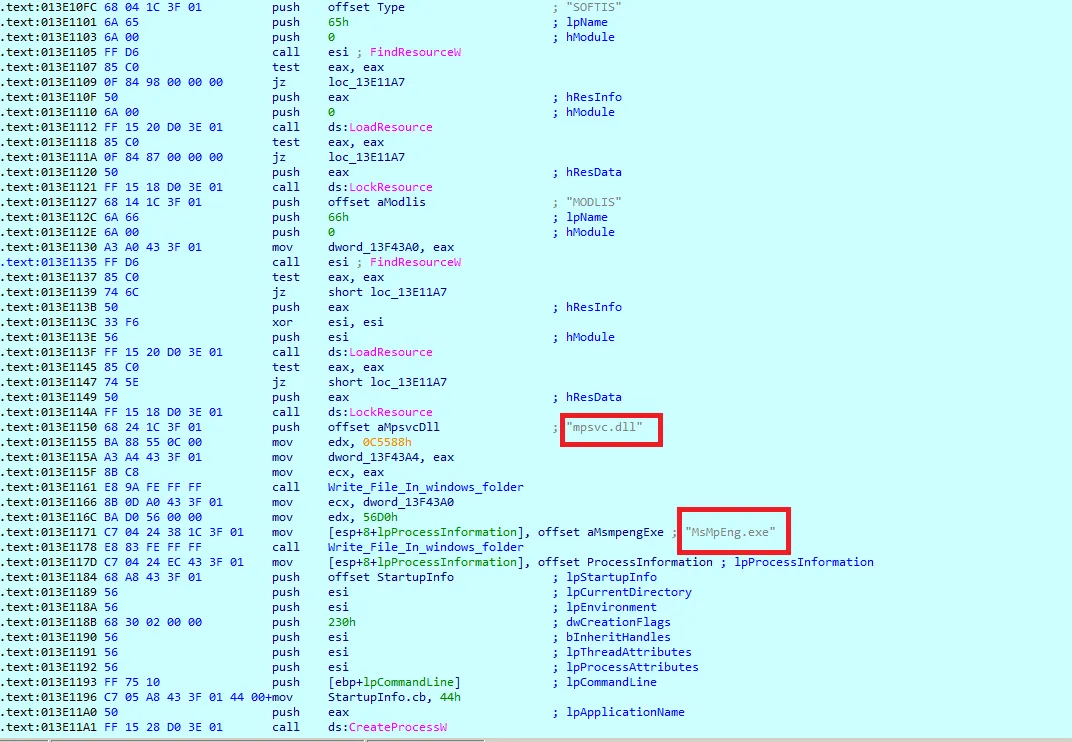
\includegraphics[width=0.8\linewidth]{rysunki/obnjdumpagenta.png}
    \caption{Miejsce w pliku binarnym \texttt{agent.exe}, w którym wywoływany jest \texttt{MsMpeng} oraz ładowany plik \texttt{.dll}\protect \footnotemark. }
    \label{fig:enter-label}
\end{figure}
\footnotetext{\url{https://ik.imagekit.io/qualys/wp-content/uploads/2021/07/Fig.-5-Write_resource_Create_process.png}}
Innym znanym RaaS jest \foreignquote{english}{DarkSide} używany przez grupę \foreignquote{english}{CARBON SPIDER}. Do niedawna skupiał się głownie na atakach maszyn Windowsowych, niedawno rozszerzając się na systemy Linux, VMware ESXi~i~vCenter~\cite{darkside}. Wirus w wersji Windowsowej obchodzi zabezpieczenia kontroli użytkownika za pomocą interfejsu \texttt{CMSTPLUA COM}\footnote{Takie obejście można dokonać programem \url{https://github.com/tijme/cmstplua-uac-bypass}}, następnie sprawdza na podstawie lokalizacji~i~języka systemu~w~celu ominięcia ataku na maszynę z jednej z byłych republik radzieckich. Program podejmuje potem następujące kroki:
\begin{enumerate}
    \item tworzy plik \texttt{LOG.<id użytkownika>.TXT} w którym przechowuje dane tymczasowe na temat progresu ataku,
    \item usuwa pliki w koszu, programy antywirusowe~i~zapewniające bezpieczeństwo oraz zamyka procesy blokujące mu dostęp do danych użytkownika,
    \item rozpoczyna szyfrowanie algorytmem \texttt{Salsa20} przy pomocy losowo wygenerowanego klucza macierzowego,
    \item klucz macierzowy jest szyfrowany zakodowanym na twardo kluczem RSA, a następnie łączony z zaszyfrowanym plikiem,
    \item pozostawia plik \texttt{README.<id użytkownika>.TXT} w którym wskazuje stronę ukrytą za TORem, na której ofiara ma dokonać płatność w BTC lub XMR.
\end{enumerate}
\begin{figure}[H]
    \centering
    
\includegraphics[width=0.75\linewidth]{rysunki/tapeta.png}
    \caption{W wyniku działania wirusa tapeta użytkownika zostaje zmieniona na taką, jak widać na obrazku\protect \footnotemark.}
    \label{fig:enter-label}
\end{figure}
\footnotetext{\url{https://staticfiles.acronis.com/images/content/5cd67c66ec1401b8e67aee9e1bb04cc4.webp}}
%%%%%%%%%%%%%%%%%%%%%%%%%%%%%%%%%%%%%%%%%%%%%%%%
\section{Istniejące techniki wykrywania i obrony przed ransomware}
\label{sec:techniques}
Niezależnie od tego czy atakujący korzysta z techniki \foreignquote{english}{living off the land} lub stara się spowodować starty w możliwie najmniejszym przedziale czasowym, 
kluczem w minimalizacji kosztów ataku ransomware najważniejsza jest szybka reakcja. Aby to osiągnąć należy podjąć inteligentną strategię, która doprowadzi do możliwie jak najwcześniejszego wykrycia ataku.
Jeśli administrator zostanie poinformowany dostatecznie wcześnie o zagrożeniu, będzie możliwa izolacja, a następnie eliminacja zagrożenia. Takie podejście w połączeniu ze 
zdyscyplinowanym harmonogramem kopii zapasowych, jest w stanie zredukować straty niemalże do zera.
\newline
Wyróżnia się trzy główne metody wykrywania ataku: poprzez sygnaturę plików, poprzez analizę nietypowego dla systemu zachowania oraz poprzez monitorowanie ruchu sieciowego~\cite{vehabovic_ransomware_2022}.
%%%%%%%%%%%%%%%%%%%%%%%%%%%%%%%%%%%%%%%%%%%%%%%%
\subsection{Wykrywanie poprzez sygnaturę plików}
Zasada działania tego typu wykrywania jest bardzo prosta. Oprogramowanie ma pewne unikalne cechy, na podstawie których wyliczana jest jego sygnatura. Do tych cech należą zakodowane na twardo nazwy domen, adresy 
IP oraz inne identyfikatory. Typowo także wykorzystywana jest wartość funkcji skrótu. Aby metoda ta mogła być skuteczna musi istnieć często aktualizowana baza danych zawierająca sygnatury wszystkich napotkanych 
typów ransomware. Niestety sposób ten jest ograniczony do wirusów napotkanych w przeszłości~i~nie jest nim możliwe wykrycie unikalnego zagrożenia.
\begin{figure}[H]
    \centering
    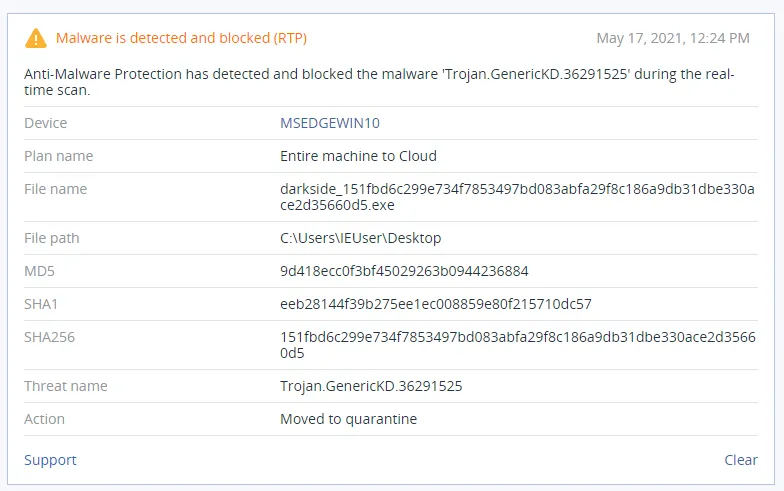
\includegraphics[width=0.65\linewidth]{rysunki/sygnatura.png}
    \caption{Tradycyjne antywirusy tak jak pokazany na obrazku Acronis, korzystają z metody wykrywania poprzez sygnaturę\protect\footnotemark.}
    \label{fig:enter-label}
\end{figure}
\footnotetext{\url{https://staticfiles.acronis.com/images/content/c110e0139779aec495bb2bd6e96ee4cd.webp}}
%%%%%%%%%%%%%%%%%%%%%%%%%%%%%%%%%%%%%%%%%%%%%%%%
\subsection{Wykrywanie poprzez analizę zachowania systemu}
\label{sec:behav}
W przeciwieństwie do wcześniej wymienionego sposobu, wykrywanie poprzez analizę zachowania system nie opiera się na sprawdzeniu treści pliku wykonywalnego, 
a na wykryciu kroków, charakterystycznych dla naruszenia bezpieczeństwa systemu. 
W przeciwieństwie do poprzedniego rozwiązania, ta metoda jest przystosowana do kontrowania techniki \foreignquote{english}{living off the land}.
Dziedzina wykrywania behawioralnego wirusów stała się m.in. obiektem badań algorytmami opartymi o sztuczną inteligencję~\cite{vehabovic_ransomware_2022}. Branych pod uwagę
może być wiele zdarzeń, z których najbardziej charakterystyczne są:
\begin{itemize}
    \item wywoływanie pewnej grupy komend powłoki systemu,
    \item pobieranie otwarto-źródłowych programów do penetracji systemów,
    \item wykorzystywanie pewnej grupy zmiennych środowiskowych jako argumenty wywołań,
    \item użycie pewnej grupy wywołań systemowych w ciągu, jedno po drugim,
    \item duży ruch w katalogach domowych użytkowników lub w \texttt{/tmp},
    \item zmiana atrybutów i właścicieli plików, katalogów czy punktów montowania dysków.
\end{itemize}
Jedną z najpowszechniejszych metod, używanym przez atakujących do powiadomienia ofiary o ataku~i~metodzie odzyskania dostępu do danych 
jest pozostawienie pliku tekstowego w miejscu łatwym do znalezienia np. w 
katalogu domowym użytkownika. Inną jest tworzenie pliku tymczasowego przechowującego 
stan zaawansowania ataku. Ze względu na to, część metod wykrywania ransomware skupia się
na wyszukiwaniu tego typu plików, na podstawie treści techniką 
\foreignquote{english}{bag-of-words}\footnote{Jest to technika przedstawienia 
tekstu w modelu nieułożonej kolekcji słów. Wykorzystuje się ją m.in. w przetwarzaniu 
języka naturalnego.} w celu odnalezienia korelacji między terminami typowymi dla 
takich dokumentów np. \foreignquote{english}{encrypted}, \foreignquote{english}{ransom}
etc.
%%%%%%%%%%%%%%%%%%%%%%%%%%%%%%%%%%%%%%%%%%%%%%%%
\subsection{Wykrywanie poprzez analizę ruchu sieciowego}
Wykrywanie poprzez analizę ruchu sieciowego polega na ograniczenia analizy behawioralnej do wyłącznie monitorowania adresatów~i~treści pakietów komunikacji sieciowej.
Szczególne zainteresowanie stanowią transfery danych do maszyn o nieznanych~i~podejrzanych adresach
oraz domenach. Zgodnie z techniką \foreignquote{english}{living off the land}, atakujący stara się
możliwe minimalizować komunikację z serwerami zewnętrznymi które mogą zostać uznane za podejrzane. Mimo to 
znakomita większość narzędzi hakerskich, jest ogólnodostępna~i~dobrze znana w branży
cyberbezpieczeństwa~i~tym samym łatwa do wykrycia~\cite{sans_secure}.  
\begin{table}[H]
    \centering
    \begin{tabular}{ll}
    \hline
    \multicolumn{1}{|l|}{Narzędzie} & \multicolumn{1}{l|}{Strona}  \\ \hline
    7zip                            & 7-zip.org                    \\
    AdFind                          & joeware.net                  \\
    Advanced IP Scanner             & advanced-ip-scanner.com      \\
    AnyDesk                         & anydesk.com                  \\
    Proces Hacker                   & processhacker.sourceforge.io \\
    rclone                          & rclone.org                   \\
    WinSCP                          & winscp.net                  
    \end{tabular}
    \caption{Tabela popularnych narzędzi wykorzystywanych w atakach ransomware\protect\footnotemark.}
\end{table}
\footnotetext{Dane pochodzą ze strony: \url{https://lots-project.com/}}
%%%%%%%%%%%%%%%%%%%%%%%%%%%%%%%%%%%%%%%%%%%%%%%%
\section{Podstawy działania systemów plików}
Struktura~i~działanie systemu plików na Linuksach jest bardzo szerokim tematem.
Na potrzeby analizy behawioralnej ataku ransomware przybliżę w tej sekcji po krótce działanie~i~
wybrane, interesujące szczegóły implementacyjne.
\subsection{Skrócony opis działania systemu plików}
Najpopularniejsze dystrybucje systemu Linux korzystają w większości z systemu plików o nazwie \texttt{ext4}.
Wprowadzony do repozytorium jądra systemowego w 2008 roku, zyskał wielkie poważanie dzięki nowoczesnej obsłudze nośników 
danych oraz ulepszeniu systemu księgowania operacji, wprodzanego w \texttt{ext3}. Księgowanie operacji w systemie plików
polega na przechowywaniu zapisów jako \emph{transakcji}. Dopiero jeśli transakcja zakończy zapisywanie na dysk, jej dane 
zostają wprowadzone na system plików~\cite{ext4}. W efekcie oznacza to, że w wypadku zaniechania działania
systemu w trakcie zapisu, transakcja zostanie cofnięta po ponownym rozruchu~i~tym samym zachowana zostanie spójność systemu plików.
\newline
Obsługa wielu rodzajów systemu plików jest możliwa dzięki istnieniu \emph{virtualnego systemu plików}. 
Jest on warstwą abstrakcji pomiędzy konkretnymi jej implmentacjami, a aplikacjami klienckimi.
Dzięki temu możliwa jest spójna~i~ujednolicona interakcja z systemem plików oraz interoperowalność między różnymi jego implementacjami~\cite{kernel}.
\begin{figure}[H]
    \centering
    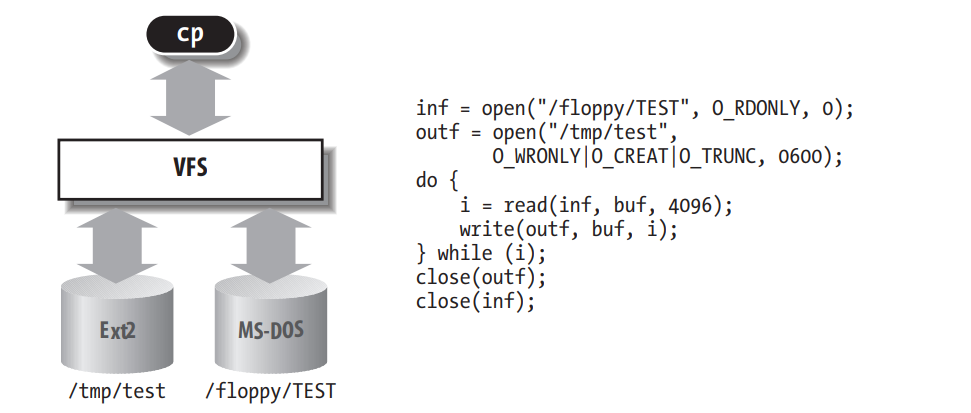
\includegraphics[width=0.9\linewidth]{rysunki/vfs.png}
    \caption{Rola wirtualnego systemu plików w operacji kopiowania\protect \footnotemark.} 
    \label{fig:enter-label}
\end{figure}
\footnotetext{\emph{Understanding Linux Kernel 3rd edition}, Figure 12-1 s. 457.}

Ogólna zasada działania wirtualnego systemu plików polegna na podmienianiu przez nią typowych wywołań systemowych
takich jak \texttt{read} lub \texttt{write} na funkcje natywne dla konkretnego systemu plików np. \texttt{ZFS} lub wcześniej wymieniony \texttt{EXT4}.
Każda implementacja musi móc przetłumaczyć swoją wewnętrzną strukturę organizacjną na model ogólny wirtualnego systemu plików~\cite{kernel}.
\begin{figure}[H]
    \centering
    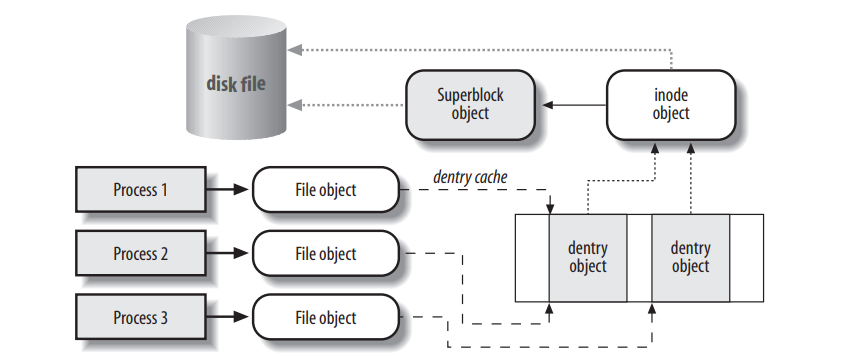
\includegraphics[width=0.9\linewidth]{rysunki/interakcjavfs.png}
    \caption{Interkacja pomiędzy procesami a objektami wirtualnego systemu plików\protect \footnotemark.} 
    \label{fig:enter-label}
\end{figure}
\footnotetext{\emph{Understanding Linux Kernel 3rd edition}, Figure 12-2 s. 460.}

Infromacje na temat interakcji pomiędzy otwartym plikiem a procesem są przechowywane~w~charakterystycznym dla procesu otwierającego plik \foreignquote{english}{file object}.
Informacje te istnieją \emph{wyłącznie}~w~pamięci jądra systemu kiedy plik jest otwarty przez proces. 
%%%%%%%%%%%%%%%%%%%%%%%%%%%%%%%%%%%%%%%%%%%%%%%%
\subsection{Monitorowanie zmian na systemie plików}
\label{sec:monitorowanie}
Jądro systemu, nie może utrzymywać zakodowanej na twardo implementacji operacji na systemie plików ze względu
na ich różnorodność. Utrzymyany jest więc indeks wskaźników do odpowienich implementacji operacji. Taka struktura komunikacji
między systemem plików a jądrem pozwala na śledzienie wywołań oprogramowaniem pośrednim. Jądro Linux zawiera w sobie dwie ciekawe
z poziomu tematu pracy impelmentacje takich \enquote{pośredników}: \foreignquote{english}{inotify subsystem} oraz \foreignquote{english}{Linux Auditing Framework}.
\subsubsection{API inotify}
\label{sec:inotify}
Podsystem inotify został stworzony z myślą o monitorowaniu oraz powiadomianiu o zmianach na dysku~\cite{love_linux_2013}. 
Jego głównym przypadkiem użycia jest automatycze aktualizowanie widoków katalogów, plików konfiuguracyjncyh, zmian
logów systemowych~i~tym podobnych. Rozwiązanie to znajduje się w kodzie źródłowym jądra Linux od sierpnia 2005 roku. Interfejs programowalny
dla tego nardzędzia zawiera się w biliotece \texttt{inotify-tools}, które zawiera w sobię również pakiet narzędzi będąch gotowymi implementacjami funkcjonalności API~\cite{biancalana_inotfy}.
\begin{lstlisting}[language=bash,
    backgroundcolor=\color{EEGold!5!white},
    caption={Przykład użycia narzędzia \texttt{inotifywait}.
    Po utworzeniu pliku ukazała się odpowiednia wiadomość},
    label={lst:helloC}]
    $ cat inotify-test.sh
    #/bin/bash
    inotifywait -m /home/user/box -e create -e moved_to |
    while read -r directory action file; do
            echo "File has been created!"
    done
    $ ./inotify-test.sh
    Setting up watches.
    Watches established.
    [1]  + 13180 suspended  ./inotify-test.sh
    $ touch box/h2
    $ fg
    [1]  + 13180 continued  ./inotify-test.sh
    File has been created!
\end{lstlisting}
Niestety rowziwązanie to nie jest perefekcyjne~i~ma swoje limity. Do nich należą:
\begin{itemize}
    \item brak wsparcia dla rekurencyjnego obserwowania ścieżek,
    \item \enquote{gubienie} niektórych wydarzeń dla starszych wersji jądra Linux,
    \item brak wsparcia niektórych wydarzeń przed wersją 5.13 jądra Linux~\cite{fanotify7},
    \item brak obserwacji dysków sieciowych.
\end{itemize}
\newpage
\subsubsection{Linux Auditing Framework}
\label{sec:auditd}
Projekt Linux Auditing Framework to podsystem wbudowany w jądro systemu Linux, którego zadaniem jest przechwytywanie,
a następnie logowanie operacji systemowych. Jego możliwości nie ograniczają się wyłacznie do 
obserwacji systemu plików. Jest on w pełni zgodny z CAPP\footnote{Controlled Access Protection Profiles to środowisko służące do niezależnej oceny, analizy i testowania produktów w celu ustanowienia wymagań bezpieczeństwa.}, a
więc może być używany jako wiarygodne źródło informacji o stanie systemu. Informacje można pobierać dzięki aplikacji
po stronie użytkownika o nazwie \texttt{auditd}. Za pomocą komponentu \texttt{auditd} możliwe jest zapisanie logów do pliku lub wysłanie ich UNIXowym gniazdkiem do innych aplikacji.
\begin{figure}[H]
    \centering
    \includegraphics[width=0.6\linewidth]{rysunki/audit.png}
    \caption{Bardzo uproszczony diagram komponentów LAF\protect\footnotemark.}
    \label{fig:enter-label}
\end{figure}
\footnotetext{\url{https://documentation.suse.com/sles/12-SP5/html/SLES-all/cha-audit-comp.html}}

Niestety bardzo ciężko jest znaleźć informacje na temat implementacji części systemu która znajduje się w jądrze, ale 
na podstawie własnej analizy kodu zawartego w repozytorium głównym projektu\footnote{Pod adresem: \url{https://github.com/linux-audit/audit-kernel}}
, w szczególności w plikach \texttt{audit.c}, \texttt{audit\_fsnotify.c} oraz \texttt{auditsc.c} w folderze \texttt{kernel}, mogę z dużą
dozą pewności stwierdzić, że infromacje wykryte tym narzędziem są wiarygodne~i~przydatne z perspektywy tematu pracy.
W branży administracji systemami jest to narzędzie dobrze znane~i~poważane dzięki możliwościom łatwej~i~bezinwazyjnej konfiguracji.
Popularne dystrybucje serwerowe takie jak Ubuntu Server, SLES, Red Hat oraz Fedora wspierają w pełni funkcjonalności
związane z monitorowaniem systemu plików. 
%%%%%%%%%%%%%%%%%%%%%%%%%%%%%%%%%%%%%%%%%%%%%%%%
\subsection{Krótka charakterystyka plików wykonywalnych}
\label{sec:elfini}
System Linux pliki wykonywalne zapisuje~i~odczytuje w formacie \texttt{ELF} czyli 
\foreignquote{english}{Executable Linking Format}~\cite{linux_foundation_tool_nodate}.
Najciekawszym elementem tego formatu, z punktu widzenia tej pracy, jest nagłówek. Mimo, że nie zawiera tak wielu informacji co
nagłówki plików wykonywalnych na systemie Windows, warto przyjrzeć się mu aby móc zidentyfikować obecność
oprogramowania złośliwego lub narzędzia typowo wykorzystywanego podczas naruszenia bezpieczeństwa systemu.
\begin{figure}[H]
    \centering
    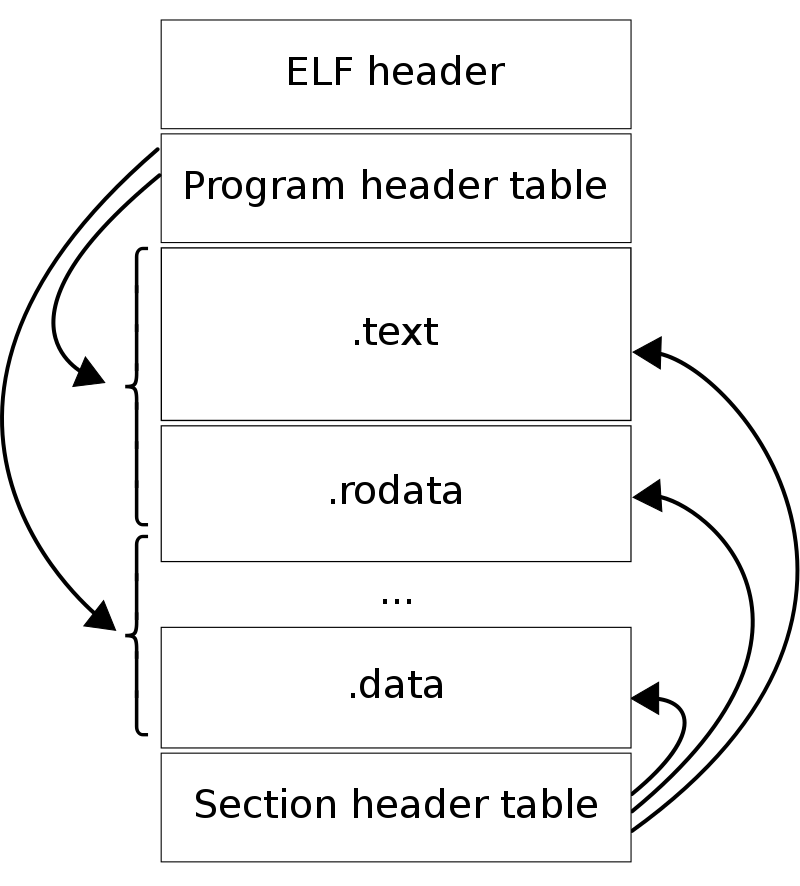
\includegraphics[width=0.45\linewidth]{rysunki/elf.png}
    \caption{Podział wewnętrzny pliku \texttt{ELF}\protect\footnotemark.}
    \label{fig:enter-label}
\end{figure}
\footnotetext{\url{https://upload.wikimedia.org/wikipedia/commons/7/77/Elf-layout--en.svg}}
W mojej opinii ciekawą sekcją jest \texttt{.note.gnu.build-id}~\cite{elfman}. Cytując
\texttt{elf(5)} Linuksowego \texttt{man pages}: \foreignquote{english}{This section is used to hold an ID that uniquely
identifies the contents of the ELF image.  Different files
with the same build ID should contain the same executable
content [...]}. Oznacza to, że można dzięki niemu \emph{zidentyfikować konkretną kompilację aplikacji}.
W przeciwieństwie do systemu Windows, gdzie typowo użytkownik pobiera już wcześniej przekompilowane pliki wykonywalne,
bardzo popularnym rozwiązaniem na Linuksach jest kompilowanie lokalnie. Wyjątkiem są zaufane repozytoria, do których dostęp
uzyskuje się przez menadżer pakietów dodawany do danej dystrybucji, np. \texttt{apt}. Mimo, że możliwa jest identyfikacja 
zawartości pliku binarnego poprzez wyliczenie jej wartości funkcji skrótu w niedługim czasie funkcją md5, identyfikator kompilacji
dla tych samych warunków kompilacji~i~zawartości kodu wykonywalnego, będzie dokładnie taki sam. Informacja ta może być wykorzystywana do
identyfikacji tego czy podejrzany plik binarny został skompilowalny lokalnie z kodu źródłowego.
\newpage
\begin{lstlisting}[language=bash,
    backgroundcolor=\color{EEGold!5!white},
    caption={Test rekompilacji aplikacji napisanej w języku Rust. Mimo ponownej kompilacji, przy braku zmiany kodu źródłowego, identyfikator pozostał ten sam.
    Można więc z dużą pewnością stwierdzić, że plik wykonywalny był skompilowalny na tej maszynie, a nie pobrany z internetu.},
    label={lst:helloC}]
    $ cargo build --release
        Finished release [optimized] target(s) in 0.13s
    $ readelf --notes target/release/linux-fs-audit | grep "Build ID"
        Build ID: ff6019887a97bedc98a8eca3267817233a13a8bc
    $ rm target/release/linux-fs-audit
    $ cargo build --release
        Finished release [optimized] target(s) in 0.04s
    $ readelf --notes target/release/linux-fs-audit | grep "Build ID"
        Build ID: ff6019887a97bedc98a8eca3267817233a13a8bc
\end{lstlisting}
%%%%%%%%%%%%%%%%%%%%%%%%%%%%%%%%%%%%%%%%%%%%%%%%
\section{Metody analizy statystyk systemu plików}
\label{sec:metody}
Wraz ze wzrostem ryzyka ataków ransomware, wzrosła też ilość prac opisujących możliwe metody wykrywania ataków
na podstawie statystyk systemowych. W tym rozdziale chciałbym wymienić~i~po krótce wytłumaczyć,~w~mojej opinii, najciekawsze z nich.
%%%%%%%%%%%%%%%%%%%%%%%%%%%%%%%%%%%%%%%%%%%%%%%%
\subsection{Analiza entropii pliku}
\label{sec:entropia}
W pracy \foreignquote{english}{Differential area analysis for ransomware
attack detection within mixed file datasets}~\cite{davies_differential_2021} przedstawiona jest 
metoda potencjalnego wykrycia tego czy plik został zaszyfrowany poprzez obliczenie entropii pliku dla różnych wielkości nagłówka.
Nagłówek~w~kontekście tej metody po prostu oznacza ilość bajtów braną pod uwagę~w~obliczaniu entropii, a niekoniecznie
twardo sprecyzowany~w~specyfikacji rodzaju pliku obszar na jego początku. Maksymalna możliwa entropia per bajt dla pliku jest równa ośmiu bitom na jeden bajt,
wartość sugerująca kompletnie losową naturę pliku. Wzór na entropię $H$~\cite{6773024} to:
$$
H(X) = - \sum_{i=1}^{n} P(x_{i})log_{2}P(x_{i})
$$
gdzie $n$ jest liczbą bajtów~w~próbce, a $P(x_{i})$ to prawdopodobieństwo wystąpienia bajtu $i$~w~strumieniu bitów.
Wyobraźmy sobie, że mamy 150 bajtowy plik który został wygenerowany losowo. Jego wykres entropi naliczonej 
od długości nagłówka $x$ będzie przypominał funkcję $log_{2}(x)$.
\begin{figure}[H]
    \centering
    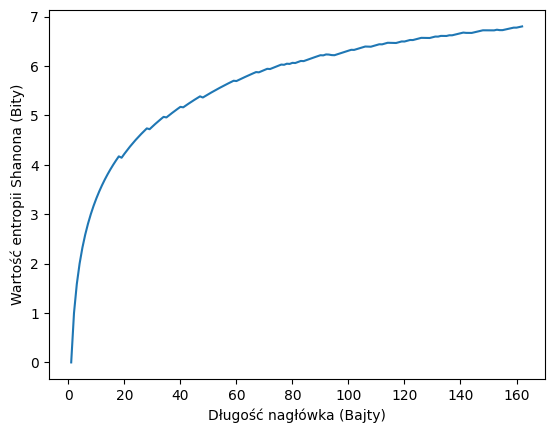
\includegraphics[width=0.65\linewidth]{rysunki/randomy.png}
    \caption{Wykres entropii od długości nagłówka dla pliku zawierającego zupełnie losowe dane.}
    \label{fig:enter-label}
\end{figure}
Dla rzeczywistych plików wartość entropii będzie rosnąć~w~mniejszym tępie, ze względu na powtarzające
się schematy~w~informacji.
\begin{figure}[H]
    \centering
    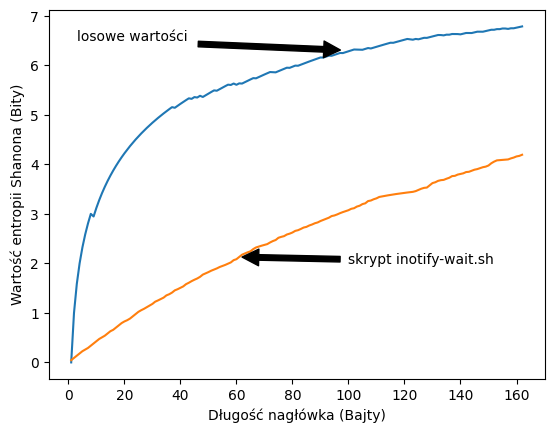
\includegraphics[width=0.65\linewidth]{rysunki/zestawienie.png}
    \caption{Zestawienie wykresów entropii od długości nagłówka. Jako plik przykładowy wybrałem skrypt~z~sekcji \hyperref[sec:monitorowanie]{Monitorowanie zmian na systemie plików}.}
    \label{fig:enter-label}
\end{figure}
Miarą tego jak duże jest prawdopodobieństwo, że plik został zaszyfrowany jest pole między tymi dwoma wykresami.
\begin{figure}[H]
    \centering
    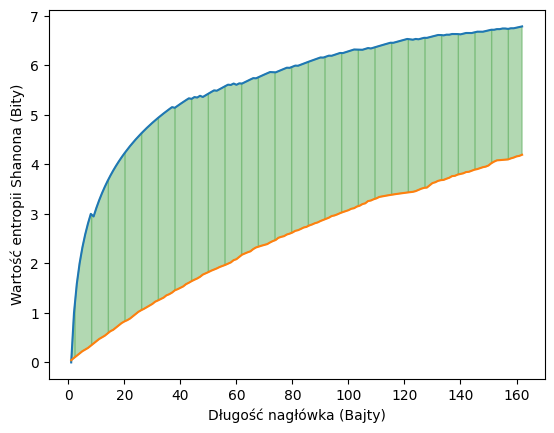
\includegraphics[width=0.7\linewidth]{rysunki/pole.png}
    \caption{Pole między wykresem losowego i rzeczywistego pliku o takich samych długościach.}
    \label{fig:enter-label}
\end{figure}
W pracy \foreignquote{english}{Differential area analysis for ransomware
attack detection within mixed file datasets}~\cite{davies_differential_2021} zasugerowane są pewne wartości klasyfikacyjne, ustalone na podstawie
dokładności wykrycia zaszyfrowanego pliku~w~zbiorach testowych.
\begin{figure}[H]
    \centering
    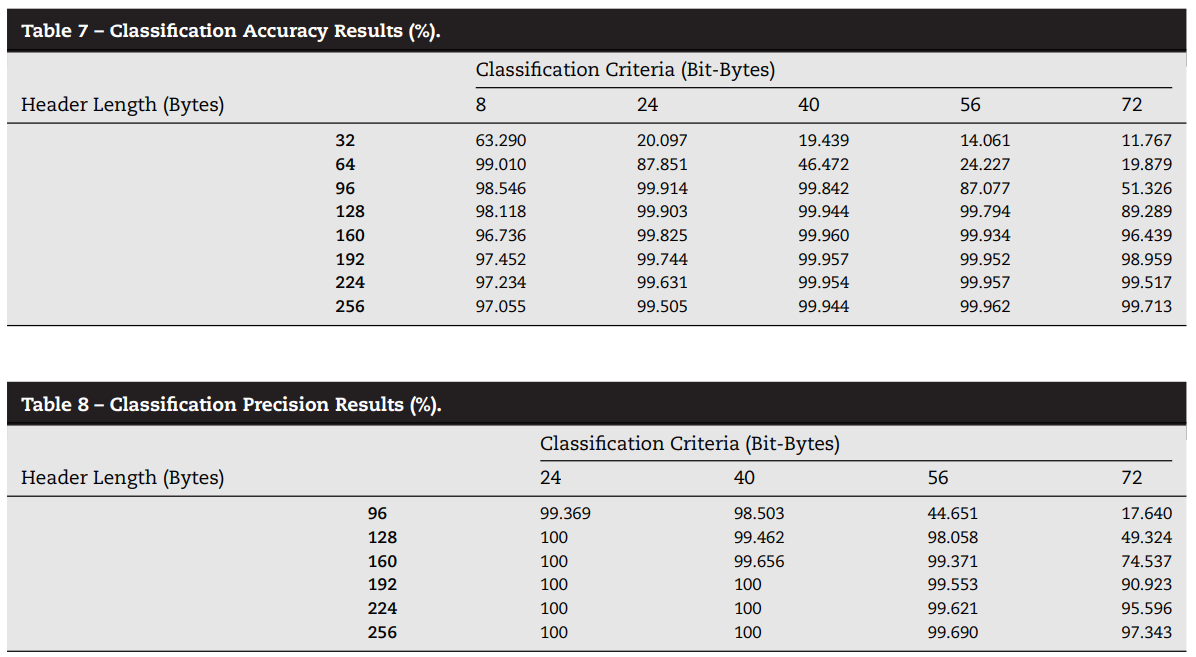
\includegraphics[width=0.85\linewidth]{rysunki/wycinek.png}
    \caption{Skuteczność dla wybranych kryteriów klasyfikacji na długość nagłówka~w~bajtach\protect\footnotemark.}
    \label{fig:enter-label}
\end{figure}
\footnotetext{\emph{Differential area analysis for ransomware
attack detection within mixed file datasets}, Table 7, Table 8, s. 11.}

Metoda ta wydaje się być bardzo obiecująca lecz jest ograniczona wymogiem wielkości pliku. Jak widać skuteczność jest lepsza dla plików o rozmiarze większym niż 32 bajty.
%%%%%%%%%%%%%%%%%%%%%%%%%%%%%%%%%%%%%%%%%%%%%%%%
\subsection{Automatyczna analiza behawioralna poprzez audyt systemu}
W pracy \foreignquote{english}{Automated Behavioral Analysis of Malware
A Case Study of WannaCry Ransomware}~\cite{8260673} opisana jest metoda identyfikacji ransomware
poprzez wyciągnięcie z logów audytu podczas rutynowego działania systemu. W przypadku tej pracy
poszukiwanie abnormalnych zachowań systemu było oparte \textbf{wyłącznie} na wiedzy o tym, że atak ma miejsce.
Aplikacja do audytowania systemu we wcześniej wymienionej pracy ma podobne możliwości do wymienionego~w~sekcji \hyperref[sec:monitorowanie]
{Monitorowanie zmian na systemie plików} Linux Auditing Framework.\newline
Przedstawiona~w~pracy metoda opera się o \foreignquote{english}{Term-Frequency-Inverse-Document-Frequency (TF-IDF)}~\cite{salton_term-weighting_1988} czyli metrykę obliczania 
wagu słów~w~oparciu o liczbę wystąpień, dostosowaną do faktu generalnie częstszego występowania niektórych słów.
Jest to metoda często wykorzysytwana~w~jako forma wydobywania informacji z tekstów m.in. \foreignquote{english}{text miningu}.
TF-IDF jest produktem dwóch statystyk: częstości występowania słowa oraz odwrotnej częstości dokumentu.
Częstotliwość występowania słowa zapisuje się wzorem:
$$
tf(t,d) = \frac{f_{t,d}}{\sum_{t'\in d}f_{t',d}}
$$
a odwrotną częstotliwość dokumentu:
$$
idf(t,D) = log \frac{N}{1 + |{d \in D : t \in d}|}
$$
gdzie słowo $t$, występujące~w~dokumencie $d$~i~wielkości zbuioru dokumentów (corpus) $N$, występuje z częstotliwością $f(t,d)$.
\newline
Niestety metoda ta nie przynosi szczególnych efektów. We wcześniej wymienionej pracy, zostały wykonane dwa eksperymenty: 
pierwszy~w~którym były wyłącznie logi z działania wirusa WannaCry oraz normalnych zachowań~w~systemie~w~osobnych dokumentach, drugi
w którym przemieszane były działania wirusa z normalnym działaniem systemu~w~tym samym dokumencie.
\begin{figure}[H]
    \centering
    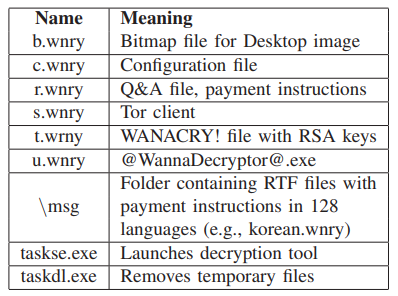
\includegraphics[width=0.3\linewidth]{rysunki/wannashit.png}
    \caption{Tabela plików tymczasowych wykorzystywanych przez wirus WannaCry\protect\footnotemark.}
    \label{fig:enter-label}
\end{figure}
\footnotetext{\emph{Automated Behavioral Analysis of Malware
A Case Study of WannaCry Ransomware}, Table I, s. 2.}

\begin{figure}[H]
    \centering
    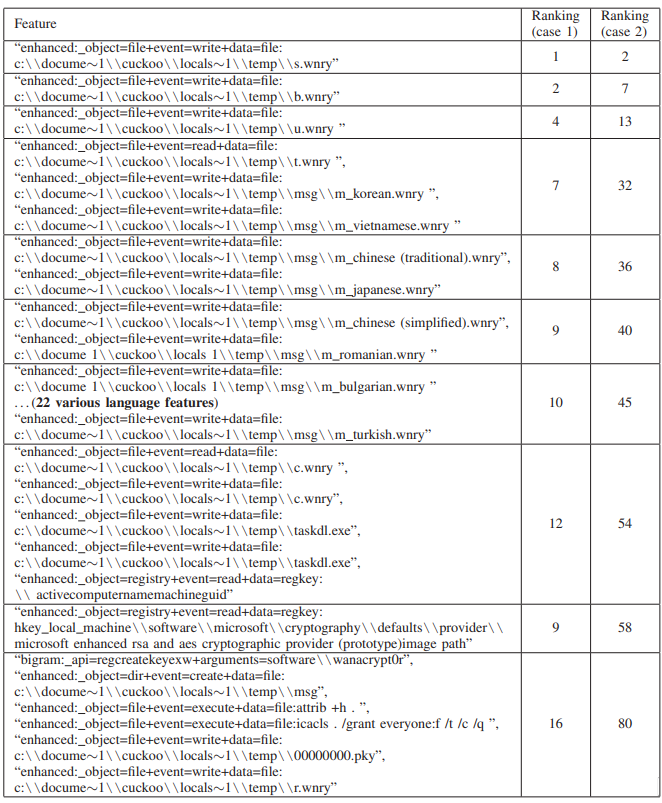
\includegraphics[width=0.85\linewidth]{rysunki/failed-exp.png}
    \caption{Tabela wyników z eksperymentu. Eksperyment pierwszy i drugi są tutaj nazwane \foreignquote{english}{case 1} i \foreignquote{english}{case 2}.
    Rankingi są wyliczone na podstawie wartości wagi TF-IDF ze wszystkich dokumentów\protect\footnotemark.}
    \label{fig:enter-label}
\end{figure}
\footnotetext{\emph{Automated Behavioral Analysis of Malware
A Case Study of WannaCry Ransomware}, Table V, s. 5.}

Jak widać z tabelki, waga informacji o działaniu ransomware znacznie zmalała po połączeniu
z logami działania systemu. Audyt systemu może być przydatny dla zaznajomionego~z~infrastrukturą
administratora lecz sama jej analiza nie jest skuteczna~w~wykrywaniu ransomware. Tym samym
informacja o dokonaniu operacji na systemie plików, sama~w~sobie nie wystarczy do wykrycia ataku.
\subsection{Analiza podobieństwa pliku wykonywalnego}
\label{sec:binaries}
Praca \foreignquote{english}{A Framework for Analyzing Ransomware using
Machine Learning}~\cite{8628743} przedstawia jako daną do przetworzenia 
przez model sztucznej inteligencji podobieńtwo cosinusowe wyliczone na 
podstawie treści wykonywalnego pliku binarnego. Podobieństwo cosinusowe
jest metodą pomiaru podobieństwa pomiędzy dwoma niezerowymi wektorami długości $n$.
Jego wartości zawierają się między zerem a jedynką. Jeśli dwa wektory mają taką samą
orientację jego wartość wynosi jeden. Dla dwóch wektorów $P$ oraz $Q$, podobieństwo 
będzie wynosić:
$$
cos(\theta) = \frac{P \cdot Q}{|P||Q|} = \frac{\sum_{i = 1}^{n} P_{i} \cdot Q_{i}}{\sqrt{\sum_{i = 1}^{n}P^{2}_{i}} \sqrt{\sum_{i = 1}^{n}Q^{2}_{i}}}
$$
W tym wypadku $P$~i~ $Q$ to dwa pliki wykonywalne, mogą to być wirusy lub zwyczajne programy codziennego użytku. Wektory te zostają utworzone na 
podstawie częstotliwości występowania instrukcji (z argumentami) kodu asemblera zdobytego z pliku binarnego, programem
\texttt{objdump}. Przykładowo dla klasycznego programu:
\begin{lstlisting}[language=C,
    backgroundcolor=\color{EEGold!5!white},
    caption={Elementarny program w C.},
    label={lst:ello}]
    #include <stdio.h>

    int main() {
        printf("Hello world!\n");
        return 0;
    }
\end{lstlisting}
do kodu asemblera będzie wyglądał w taki sposób:
\begin{lstlisting}[language=C,
    backgroundcolor=\color{EEGold!5!white},
    caption={Fragment asemblerowego kodu programu z listingu 3.},
    label={lst:ello2}]
000000000040104e <_start>:
  40104e:	f3 0f 1e fa          	endbr64
  401052:	66 90                	xchg   %ax,%ax
  401054:	31 ed                	xor    %ebp,%ebp
  401056:	49 89 d1             	mov    %rdx,%r9
  401059:	5e                   	pop    %rsi
  40105a:	48 89 e2             	mov    %rsp,%rdx
  40105d:	48 83 e4 f0          	and    $0xfffffffffffffff0,%rsp
  401061:	50                   	push   %rax
  401062:	54                   	push   %rsp
  401063:	45 31 c0             	xor    %r8d,%r8d
  401066:	31 c9                	xor    %ecx,%ecx
  401068:	48 c7 c7 46 11 40 00 	mov    $0x401146,%rdi
  40106f:	ff 15 53 2f 00 00    	call   *0x2f53(%rip) 
  401075:	f4                   	hlt
  401076:	66 2e 0f 1f 84 00 00 	cs nopw 0x0(%rax,%rax,1)
  40107d:	00 00 00 
\end{lstlisting}
Aby przedstawić jak wygląda ta metoda, spreparowałem plik zawierający wyłącznie instrukcje asemblerowe z argumentami.
Z nich wyliczyłem częstość występowania poszczególnych słów, a następnie wyliczyłem współczynnik podobieństwa ze wzoru przedstawionego wcześniej. 
Dany jest program z \hyperref[lst:ello]{listingu 3} oraz:
\begin{lstlisting}[language=C,
    backgroundcolor=\color{EEGold!5!white},
    caption={Program podobny do programu z listingu 3. Jedyną różnicą jest obecność zmiennej $i$.},
    label={lst:helloC}]
    #include <stdio.h>

    int main() {
        int i = 2;
        printf("Hello %d!\n",i);
        return 0;
    }
\end{lstlisting}
Ich podobieństwo wyliczone ze wcześniej wymienionego wzoru wynosi $cos(\theta) = 0.996289145765327$, czyli jest bardzo duże co pokrywa się z oczekiwaniami.
Jego wartość \emph{odzwierciedla} różnicę pomiędzy dwoma plikami, więc miara ta jest czuła na nawet niewielkie zmiany.
\begin{figure}[H]
    \centering
    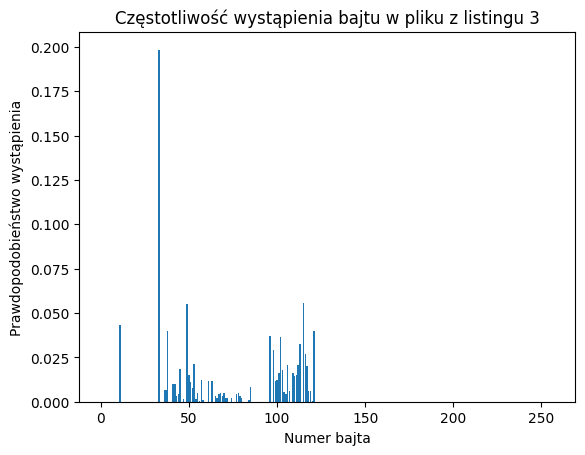
\includegraphics[width=0.69\linewidth]{rysunki/p1.png}
    \caption{Prawdopodobieństwa wystąpienia bajtów o konkretnej wartości w pliku z listingu 3.}
    \label{fig:enter-label}
\end{figure}
\begin{figure}[H]
    \centering
    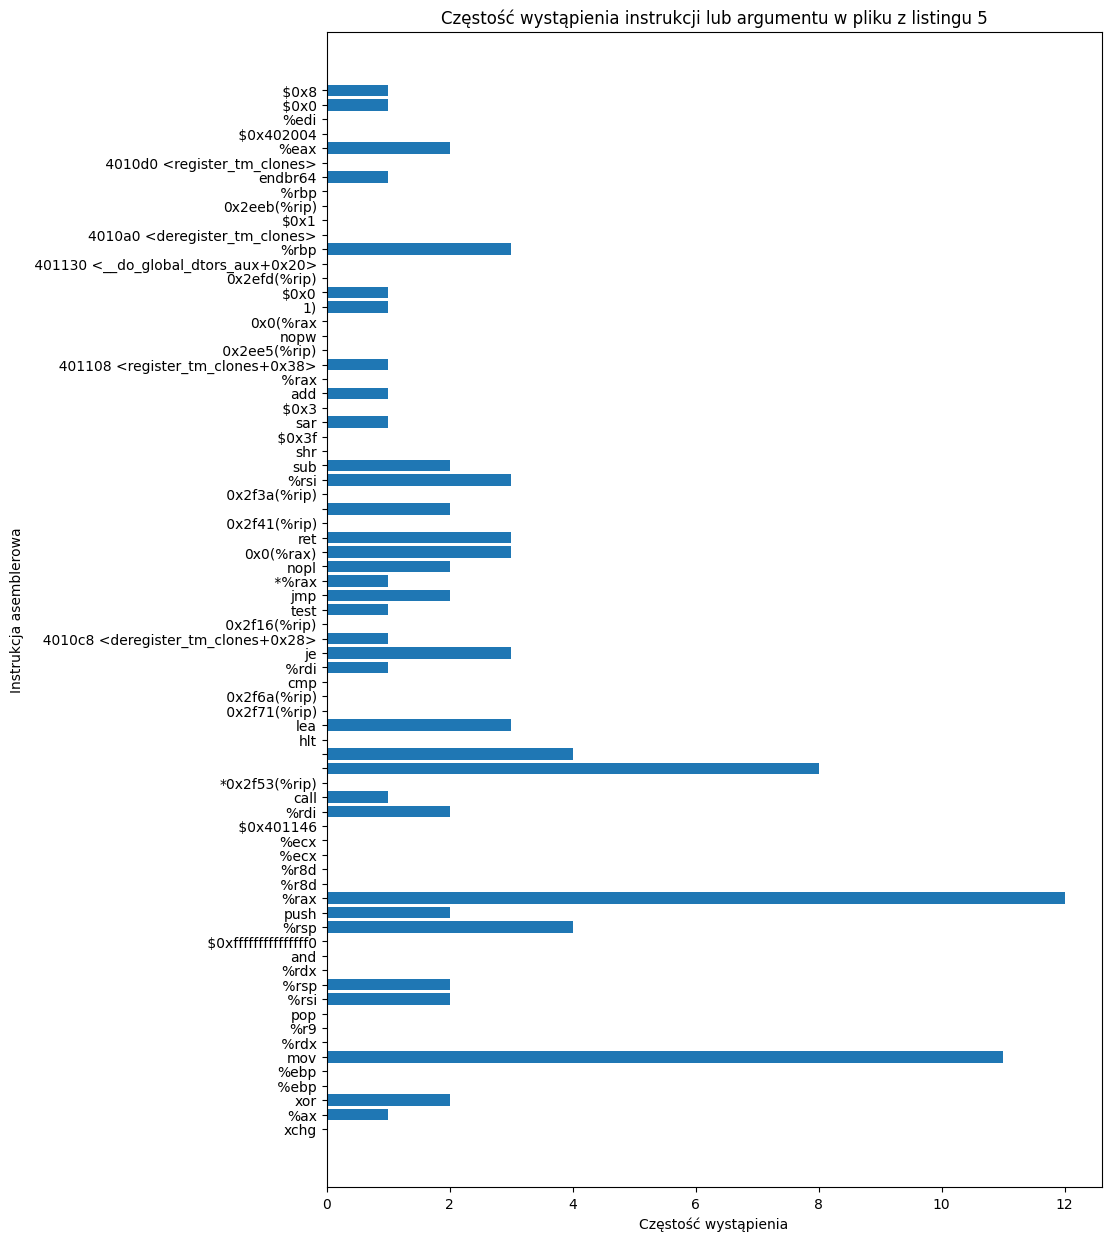
\includegraphics[width=0.69\linewidth]{rysunki/p2.png}
    \caption{Prawdopodobieństwa wystąpienia bajtów o konkretnej wartości w pliku z listingu 5.}
    \label{fig:enter-label}
\end{figure}
Jest to obiecująca metoda, która w przeciwieństwie do sprawdzania sygnatury pliku funkcją skrótu, adaptuje się do małych~i~średnich zmian w historycznie występujących zagrożeniach.
\afterpage{\blankpage}

%\input{tekst/donapisania}

\chapter{Niebanalny tytuł kolejnego rozdziału}



\chapter{Podsumowanie}
\label{ch:podsumowanie}
\section{Główne osiągnięcia pracy}
\section{Ograniczenia proponowanej metody}
\section{Propozycje dalszego rozwoju i doskonalenia systemu}


    % Bibliografia - musi być
    % Bibliography - must exist
    \bibliografia

    % Strony końcowe - można zakomentować, jeśli zbędne
    % Additional pages - comment out if not needed
    
    % Wykaz symboli i skrótów - patrz opis w tekście przykładowym
    %\acronymslist
    % Spis rysunków
    \listoffigures
    % Spis tabel
    \listoftables
    % Załączniki (plik appendices.tex)
    \easyappendices
\end{document}
%%%%%%%%%%%%%%%%%%%%%%%%%%%%%%%%%%%%%%%%%%%%%%%%%%%%%%%%%%%%%%%%%%%%%%%%%%%

